\chapter{Introduction}

Automated testing has never been an outdated problem in the mobile application development process. There are over 2,500 manufacturer models and over 100 mobile operating system versions \cite{crittercism}. Daily developed mobile applications need to be tested in a wide range of phone designs and platforms. These situations result in an enormous amount of testing scenarios and require an effective industrial testing series. Current software-based testing method has shown some advantages, but there are still some issues demanded to be dealt with.

The problem of present testing method is that only software aspect is considered. The tester can run test cases perfectly in software, regardless hardware's failure like button or touch screen malfunction. Otherwise, each phone operating system requires a different corresponding testing framework. These factors conspire to make the cross-platform mobile application testing very challenging. \nocite{weinman_thesis}

We propose a new approach that in its design, software and hardware testing are more integrated. Applying image processing technologies, our system can detect the content of phone screens and produce actions on them. These actions are performed directly on target phone by Delta robot. Robotics testing gives us a less invasive way of mobile testing that does not require special software on the target phone. In addition, the testing series can be applied to any mobile phone operating systems without a doubt.

\section{System overview}
The system overview and design are described below in Figure \ref{fig:sys_overview_hw} and \ref{fig:sys_overview}.

	\begin{figure}
		\centering
		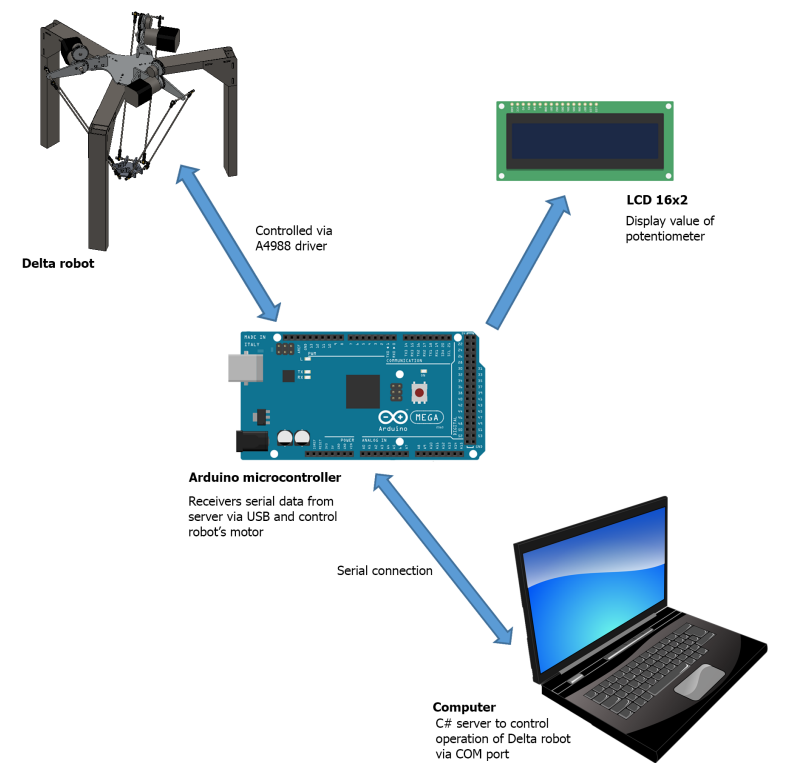
\includegraphics[scale=0.7]{Chapters/Fig/sys_overview_hw.png}
		\caption{System overview}
		\label{fig:sys_overview_hw}
	\end{figure}

Our system contains two parts: hardware and software.
Hardware part includes Delta robot with its controllers. This part which is designed and manufactured by my partner, Nguyen Tien \textit{Huong}, takes responsibility for contacting with the mobile phone, as a human doing.
The software framework receives the phone's screen and analyzes data for deciding what action to be executed by the Delta robot.
These two parts are connected by a controller module which provides a command interface for the software program to communicate with the hardware layer.

In this thesis, I construct testing software framework with screen reading modules and testing script manager. In experiments, I let the robot perform several tests on our phones with some mobile applications.

	\begin{figure}[H]
		\centering
		\includegraphics[scale=0.7]{Chapters/Fig/sys_overview.png}
		\caption{System design}
		\label{fig:sys_overview}
	\end{figure}

\section{Goals of the thesis}
To achieve desired testing framework, the mission is to complete following tasks:
	\begin{itemize}
		\item[--] Software applications
        	\begin{itemize}
				\item[+] To detect and recognize mobile phone screen's components (button, selection box, text, keyboard).
				\item[+] To generate test scripts compactly and conveniently.
			\end{itemize}
		\item[--] Hardware requirements
        	\begin{itemize}
				\item[+] To perform a testing process on the robot with gestures: tap, tap and hold, swipe,... on the phone.
				\item[+] Every action must be executed precisely in the target position.
			\end{itemize}
	\end{itemize}

\section{Outline of thesis}
In the first three chapters, I will be dealing with technologies and tools supporting testing process which include theoretical background and implementation in the project. The next chapter describes practical experiments with the system and our evaluation of the results. The last chapter brings our conclusion on what we have done and our vision of the future researches.

The first component to be covered is mobile phone screen content recognition module. The following chapter describes the image processing algorithms used for understanding the meaning of the screen. 

When the system is aware of the contents of the screen, it calls the second component, test script manager, for generating actions with these contents. Chapter \ref{ch:test_script} will clarify the testing script's structure and give some specific examples that we use for our experiments.

Finally, every single component are combined in a unified program. The implementation of this program is stated in Chapter \ref{ch:implement}.

In general, the whole thesis aims mainly to establish a testing framework on mobile phone using robotic technology. \nocite{radim_thesis}
